Cancer is a progressive and complex multi-step process within a living system. Oncogenesis is usually driven by somatic lesions which lead to mutations that eventually confer advantages to the affected cell. A cancerous cell reveals an accumulation of the alterations acquired along with its life.
\\

Many studies \cite{Rifai2006ProteinUtility}\footnote{In order to avoid over-referencing, the linked document gathers several studies focusing on biomarkers.} focus on identifying \textit{biomarkers}, alterations which identify a condition to differentiate cancer types. Biomarkers can lead the investigation to drug targets which to action clinically.

However, the efficiency of biomarker-seeking methods in clinical trials is widely unpredictable. Cancer's evolution is highly dependent on the patient’s genome and environment \cite{Yates2012EvolutionGenome}, and they both build a niche where cancer type divergence occurs. There is evidence that several individuals diagnosed under the same condition, have different prognosis due to heterogeneous cells within cancer \cite{Gao2016LossTherapy} \cite{Zaretsky2016MutationsMelanoma}, which eventually leads to relapse due to the patient's organism's unresponsiveness to treatment.

\subsection{Gene chronological order}
Currently, cancer types can be identified based on molecular and genetic information, e.g. Breast cancer has 4 genetically different known subtypes: Luminal A, Luminal B, Triple-negative/basal-like, and HER2-enriched. They accumulate \textit{different mutations}, and therefore drive to divergent behaviors and prognosis.

On the other hand, subtype communities can also arise due to the fact the \textit{same mutations} have been acquired by its cells, but the alterations occurred in a different order.
Then, does this chronological order affect the evolution of the disease?
\\

This work bases its hypotheses on the chronological order of mutation events assumption. Hence, cancer evolution can be seen as a tree diagram\footnote{We expect a modeling similar to a phylogenetic tree, in which divergence and evolution from a common ancestor have a tree-like shape. The main definition of a \emph{tree} in graph theory does not allow for cycles or convergence of any kind. Here we refer to phenotypical divergence, i.e. an accumulation of mutations that eventually deliver different outcomes. Genetically, only clones evolving in the same branch would remain genetically similar and, as a consequence, distorted.}, based on the order the alteration has been acquired. As a consequence, subtype classification, and evolution prediction could be done using the diagram's branches.

\subsection{Pathway-driven ordering}
A common belief is that a cell needs to acquire certain mutation-driven properties in order to become cancerogenic. Generally, these include a potential capacity of avoiding apoptosis, unlimited replication power, unresponsiveness to (external) signals, angiogenesis, and other tissue invasions, among others \cite{Hanahan2011HallmarksGeneration}. Cell’s pathways regulate such biological functions, and any dysregulation event within them trigger malfunctions.
\\

Individual gene mutation and consequent defective function, have a cascade effect on the pathway the gene is related to (Figure \ref{fig:gp}). The alteration will eventually distort any system which interacts with it.

Studies like \cite{Gerstung2011TheTumorigenesis} found an average of 70\% pathway alteration frequency in all analyzed samples across colorectal carcinoma, pancreatic cancer, and glioblastoma conditions. Therefore, selective pressure ultimately impacts at a pathway level.
\\

\begin{figure}
    \centering
    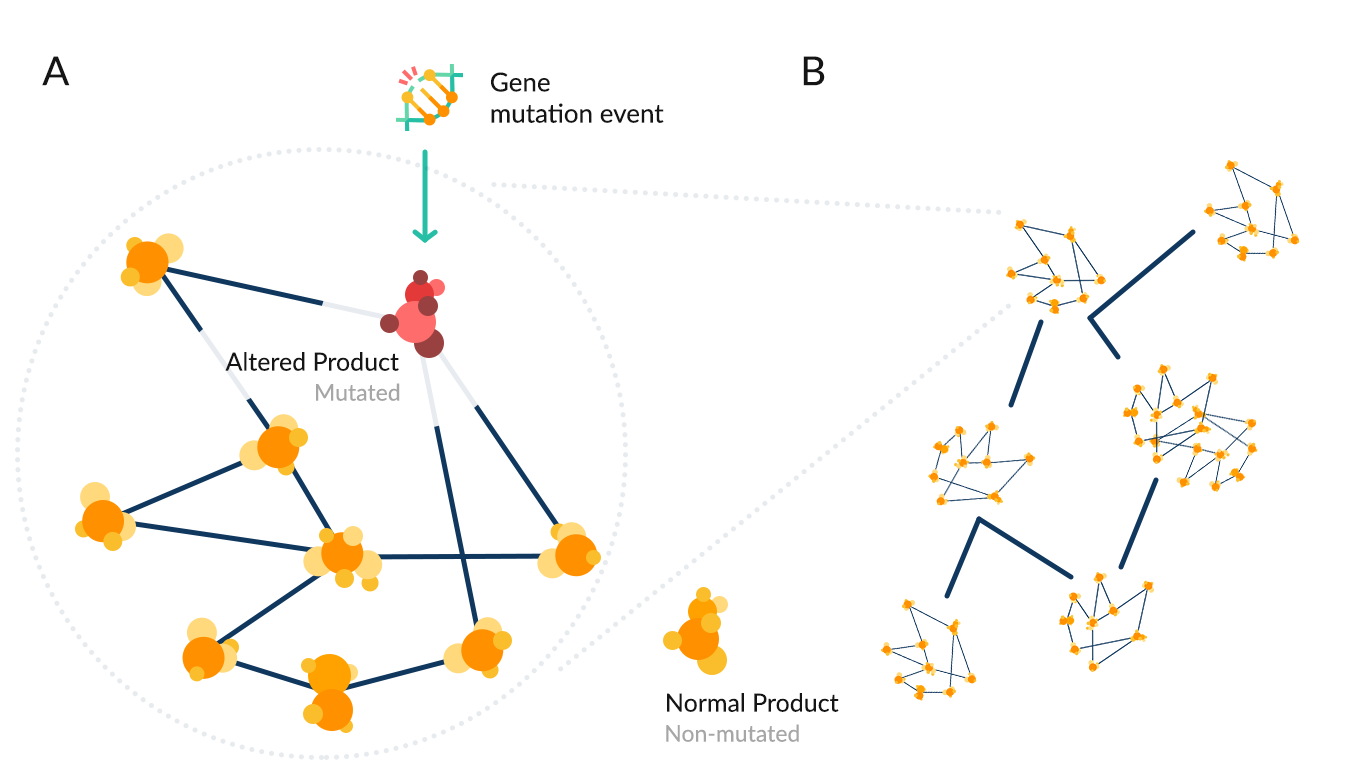
\includegraphics[width=\linewidth]{images/GP.png}
    \caption{Schema relating gene- and pathway-based order approaches. (A) displays the known fact of a mutational event disrupting the regular behavior of all the items interacting with its altered product. (B) shows how the previous dysregulation, which acts at the pathway level, has triggers deeper consequences across all related pathways.}
    \label{fig:gp}
\end{figure}

Nevertheless, pathway dysregulation might differ slightly from one patient to another \cite{Ulitsky2010DEGAS:Diseases}. The same cancer type diagnosed in different patients can result in vast heterogeneity of cases due to different dysregulation events trajectories (within the same or different pathways) \cite{Khakabimamaghani2019UncoveringDysregulation}.

Consequently, we can ask: Is mutation order responsible for different pathways dysregulation among patients under the same diagnosis?

Previous individuals' environment exposure (nutrition, smoking, ambient factors, etc.) \cite{Jung2007EnvironmentalGenome} already sets different starting points from which a condition can be developed, i.e. the genetic scenario influences an individual’s evolution, both as a healthy organism or as a diseased one. Thus alterations occurring in a different order could be influential in this setup, and prominent in clinical follow-up.

\subsection{Inheritance implications in the picture}
Notwithstanding, aside from somatic mutations, the genetic luggage we carry is also influential in cancer prognosis. Inherited mutations cause 5-10\% of family cancer syndromes, making certain individuals more prone to develop a condition.
\\

Labeling as \textit{early} in the chronology a mutation event which usually belongs to \textit{late} stages of cancer,  would be an example of the consequences.  Assuming the alteration might have been inherited from a parent, at the eyes of the analysis it \textit{has happened} in the earliest stages. Transferred to gene and/or pathway ordering, it would mean events occurring in an exceptional\footnote{DNA/Gene alterations can already be considered exceptional. The abnormality we mention is related to \emph{time expectancy}, i.e. we expect A happening before B, but B occurs before A.} order interfere with the order assumptions proposed above.

We then ask: Do inherited mutations have an impact on the order genes suffer mutations? Is it larger than somatic mutations?
\\

We can hypothesize that inheritance acts as a barrier for tracing an order of alterations, since heritage is commonly not taken into consideration in the analysis. Any model based on chronology which experiences reordering in its items will fail at delivering a solid display of the events.